\documentclass[8pt]{beamer}
\usepackage[cache=false]{minted}
\usepackage[utf8x]{inputenc}
\usepackage{hyperref}
\usepackage{fontawesome}
\usepackage{graphicx}
\usepackage[english,ngerman]{babel}
\usepackage{bussproofs}
\usepackage{dsfont}
\usepackage[all]{xy}

% ------------------------------------------------------------------------------
% Use the beautiful metropolis beamer template
% ------------------------------------------------------------------------------
\usepackage[T1]{fontenc}
\usepackage{fontawesome}
\usepackage{FiraSans}
\newtheorem{defin}{Definition}
\newtheorem{theor}{Theorem}
\newtheorem{prop}{Proposition}
\mode<presentation>
{
  \usetheme[progressbar=foot,numbering=fraction,background=light]{metropolis}
  \usecolortheme{default} % or try albatross, beaver, crane, ...
  \usefonttheme{default}  % or try serif, structurebold, ...
  \setbeamertemplate{navigation symbols}{}
  \setbeamertemplate{caption}[numbered]
  %\setbeamertemplate{frame footer}{My custom footer}
}

% ------------------------------------------------------------------------------
% beamer doesn't have texttt defined, but I usually want it anyway
% ------------------------------------------------------------------------------
\let\textttorig\texttt
\renewcommand<>{\texttt}[1]{%
  \only#2{\textttorig{#1}}%
}

% ------------------------------------------------------------------------------
% minted
% ------------------------------------------------------------------------------


% ------------------------------------------------------------------------------
% tcolorbox / tcblisting
% ------------------------------------------------------------------------------
\usepackage{xcolor}
\definecolor{codecolor}{HTML}{FFC300}

\usepackage{tcolorbox}
\tcbuselibrary{most,listingsutf8,minted}

\tcbset{tcbox width=auto,left=1mm,top=1mm,bottom=1mm,
right=1mm,boxsep=1mm,middle=1pt}

\newtcblisting{myr}[1]{colback=codecolor!5,colframe=codecolor!80!black,listing only,
minted options={numbers=left, style=tcblatex,fontsize=\tiny,breaklines,autogobble,linenos,numbersep=3mm},
left=5mm,enhanced,
title=#1, fonttitle=\bfseries,
listing engine=minted,minted language=r}


% ------------------------------------------------------------------------------
% Listings
% ------------------------------------------------------------------------------
\definecolor{mygreen}{HTML}{37980D}
\definecolor{myblue}{HTML}{0D089F}
\definecolor{myred}{HTML}{98290D}

\usepackage{listings}

% the following is optional to configure custom highlighting
\lstdefinelanguage{XML}
{
  morestring=[b]",
  morecomment=[s]{<!--}{-->},
  morestring=[s]{>}{<},
  morekeywords={ref,xmlns,version,type,canonicalRef,metr,real,target}% list your attributes here
}

\lstdefinestyle{myxml}{
language=XML,
showspaces=false,
showtabs=false,
basicstyle=\ttfamily,
columns=fullflexible,
breaklines=true,
showstringspaces=false,
breakatwhitespace=true,
escapeinside={(*@}{@*)},
basicstyle=\color{mygreen}\ttfamily,%\footnotesize,
stringstyle=\color{myred},
commentstyle=\color{myblue}\upshape,
keywordstyle=\color{myblue}\bfseries,
}

\setbeamercolor{emph}{fg=blue}
\renewcommand<>{\emph}[1]{%
  {\usebeamercolor[fg]{emph}\only#2{\itshape}#1}%
}

% ------------------------------------------------------------------------------
% The Document
% ------------------------------------------------------------------------------
\title{Intuitionistic epistemic logic categorically and algebraically}
\author{Daniel Rogozin \\ UCL}
\date{PPLV seminar \\ The 24th of March 2023}
\begin{document}

\maketitle

\section{Introduction}

\begin{frame}
\frametitle{Intuitionistic modal logic: the big picture}
\begin{itemize}
\item As it is well known, modal logic extends classical logic with modal operators.
\item Applications: topology, proof theory, formal verification, ontologies, etc.
\item Intuitionistic modal logic is a version of modal logic where the underlying logic is the intuitionistic one.
\item Possible topics where intuitionistic modal logic is of interest:
\begin{itemize}
\item Constructive necessity, provability in intuitionistic arithmetic, intuitionistic knowledge, etc.
\item Model theory: the finite model property, canonicity \`a la Salqvist, definability \`a la Thomason-Goldblatt, etc.
\item Representation theory: general descriptive frames, Esakia duality, etc.
\end{itemize}
\end{itemize}
\onslide<2->{
See this summary paper to have the big picture in more detail
\begin{itemize}
\item Frank Wolter and Michael Zakharyaschev. Intuitionistic Modal Logic, 1999.
\end{itemize}
}
\end{frame}


\begin{frame}
\frametitle{Modalities type theoretically}

\begin{itemize}
\item Type theory deals with a computation every value in which is annotated with the corresponding data type. Type theory is closely connected with intuitionistic logic and constructive proofs through the Curry-Howard correspondence.
\item One can extend Curry-Howard to intuitionistic modal logic and study modal operators within the “types-as-formulas” and “proofs-as-terms” paradigm.
\item Here we think of modal types as abstract data types of action, which is of interest for functional programming.
\end{itemize}

\onslide<2->{
See the following:
\begin{itemize}
\item Gianluigi Bellin, Valeria De Paiva and Eike Ritter. Extended Curry-Howard Correspondence for a Basic Constructive Modal Logic, 2003
\item Frank Pfenning and Rowan Davies. A Judgmental Reconstruction of Modal Logic, 2000.
\item Peter Nicholas Benton, Gavin M. Bierman, Valeria de Paiva. Computational types from a logical perspective, 1998.
\item David Corfield. Modal homotopy type theory: The prospect of a new logic for philosophy, 2020.
\end{itemize}
}

\end{frame}

\section{Modal type theory based on ${\bf IEL}^-$}

\begin{frame}
\frametitle{Bridges with functional programming}
\end{frame}

\begin{frame}
\frametitle{The definition of the type theory}
\end{frame}

\begin{frame}
\frametitle{Strong normalisation}
\end{frame}

\begin{frame}
\frametitle{The Church-Rosser property}
\end{frame}

\section{Categorical completeness}

\begin{frame}
\frametitle{Category theory}

Now I am going to be like the guy from the right.
\begin{center}
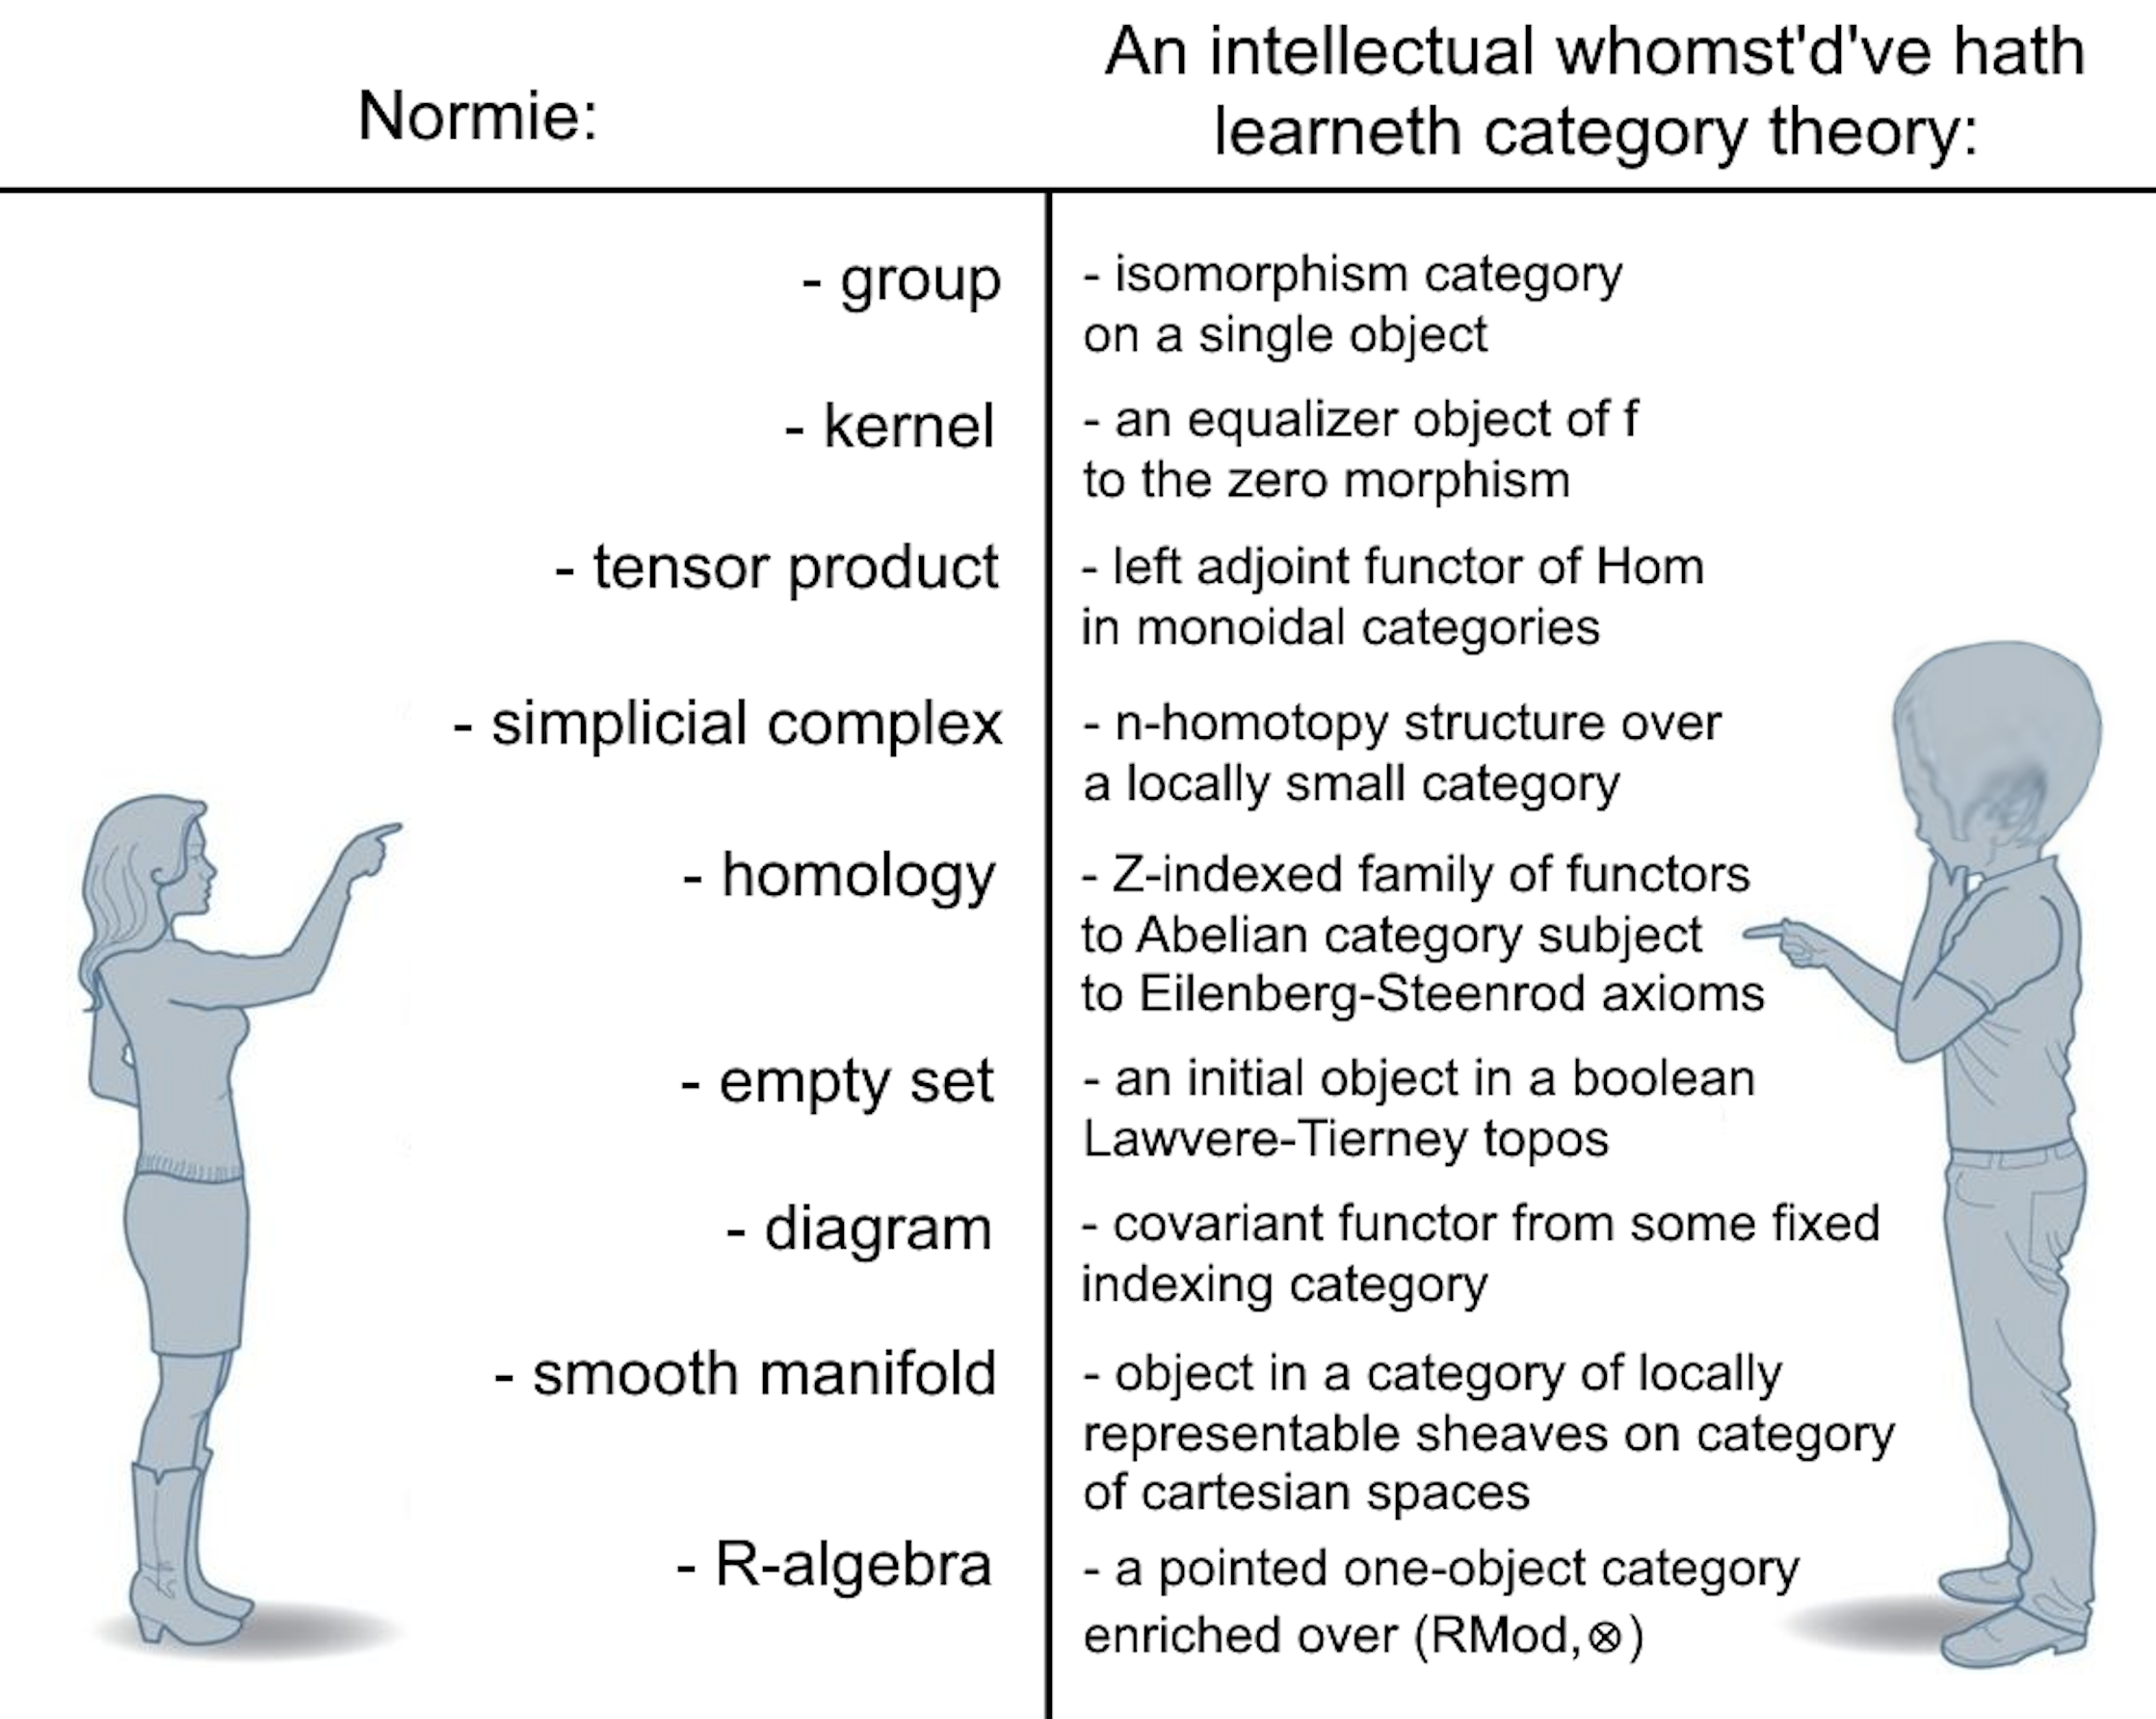
\includegraphics[scale=0.225]{meme.png}
\end{center}

\end{frame}

\begin{frame}
\frametitle{General concepts: Category}
Recall that a category $\mathcal{C}$ consists of:
\begin{itemize}
\item A class of objects $\operatorname{Ob}(\mathcal{C}) = \{ A, B, C, \dots \}$,
\item A class of morphisms $\mathcal{C}(A, B)$ for each $A, B \in \operatorname{Ob}(\mathcal{C})$, where $f : A \to B$ iff $f \in \mathcal{C}(A, B)$,
\item For $f : A \to B$ and $g : B \to C$, then $g \circ f : A \to C$ and $h \circ (g \circ f) = (h \circ g) \circ f$ for each $f, g, h$ having an appropriate domain and codomain,
\item For each $A, B \in \operatorname{Ob}(\mathcal{C})$ we have identity morphisms such that for each $f : A \to B$ $f \circ id_A = f$ and $id_B \circ g = g$.
\end{itemize}

Some examples:
\begin{itemize}
\item ${\bf Set}$, the category of all sets and all functions betweem them,
\item ${\bf Top}$, the category of all topological spaces and continuous maps,
\item ${\bf Vect}_k$, the category of vector spaces over a field $k$ and linear maps,
\item $(P, \leq)$, any poset where $a \to b$ exists iff $a \leq b$,
\item Any monoid (as well as a group) is a category, where $\operatorname{Ob}(\mathcal{C})$ is a singleton set (Cayley's theorem).
\item etc.
\end{itemize}
\end{frame}

\begin{frame}
\frametitle{General concepts: Functor}

Intuitively, a functor is a morphism of category. Rigorously, let $\mathcal{C}$ and $\mathcal{D}$ be categories, a functor $F : \mathcal{C} \to \mathcal{D}$ is a ``function'' such that:
\begin{itemize}
\item Each $A \in \operatorname{Ob}(\mathcal{C})$ maps to $F A \in \operatorname{Ob}(\mathcal{D})$,
\item Each $f : A \to B$ in $\mathcal{C}$ maps to $F f : F A \to F B$ in $\mathcal{D}$,
\item $F (g \circ f) = F g \circ F f$ for each $f$ and $g$.
\end{itemize}

Some examples:
\begin{itemize}
\item The powerset functor $\mathcal{P} : {\bf Set} \to {\bf Set}$ such that $\mathcal{P} : A \mapsto 2^{A}$,
\item The abelianisation functor $Ab : {\bf Group} \to {\bf Ab}$ such that $Ab : G \mapsto G / [G, G]$,
\item The spectrum functor $\operatorname{Spec} : {\bf Ring}^{op} \to {\bf Top}$ that maps every commutative ring to its Zariski space,
\item ${\bf Field} \to {\bf Ring}$ such that $K \mapsto K[X]$,
\item $\pi_1 : {\bf Top}_* \to {\bf Group}$ maps every topological space with a base point to its fundamental group, for example, $\pi_1(S) = \mathbb{Z}$ (up to isomorphism).
\item etc.
\end{itemize}
\end{frame}

\begin{frame}
\frametitle{General concepts: Natural transformation}
A natural transformation is a functor morphism. Let $\mathcal{C}, \mathcal{D}$ be categories and $F, G : \mathcal{C} \to \mathcal{D}$ functors. A natural tranformation $\theta : F \Rightarrow G$ is a collection of morphisms $\theta_A : F A \to G A$ in $\mathcal{D}$ making the following square commute for each $f : A \to B$ and $A, B \in \operatorname{Ob}(\mathcal{C})$:
\centerline{
\xymatrix{
F A \ar[rr]^{F f} \ar[d]_{\theta_A} && F B \ar[d]^{\theta_B} \\
G A \ar[rr]_{G f} && G B
}}

\onslide<2->{
An example:

Let $det_M$ be the determinant of the $n \times n$ matrix $M \in \operatorname{GL}_n K$ with entries from a field $K$ and $K^*$ is the multiplicative group of $K$. Both $\operatorname{GL}_n$ and $*$ are functors from the category of fields to the category of groups, and $det_M : \operatorname{GL}_n K \to K^*$ is a morphism of groups and it is natural:
\centerline{
\xymatrix{
\operatorname{GL}_n K \ar[rr]^{f} \ar[d]_{det M} && \operatorname{GL}_n K' \ar[d]^{det M'} \\
K^* \ar[rr]_{f^*} && {K'}^*
}
}
}
\end{frame}

\begin{frame}
\frametitle{Cartesian closed categories}

A category is \emph{cartesian closed} is there are objects $\mathds{1}$, $B^A$ and $A \times B$ such that:
\begin{itemize}
\item $|\mathcal{C}(A, \mathds{1})| = 1$ for each $A \in \operatorname{Ob}(A)$,
\item The following diagrams commute:
\centerline{
\xymatrix{
& C \ar[dl]_{f} \ar[dr]^{g} \ar[d]^{(f, g)} && C^B \times B \ar[rr]^{ev} && C \\
A & \ar[l]^{\pi_1} A \times B \ar[r]_{\pi_2} & B & A \times B \ar[urr]_{f} \ar[u]^{\hat{f} \times id_B}
}
}
\end{itemize}
The second diagram can be reformulated as (compare with the definition of implication in Heyting algebras):
\begin{center}
$\mathcal{C}(A \times B, C) \simeq \mathcal{C}(A, C^B)$
\end{center}

\onslide<2->{
Some examples:
\begin{itemize}
\item ${\bf Set}$,
\item Every Heyting algebra,
\item The category of $G$-sets for a group $G$ (the category of group actions),
\item The category of simplicial sets (which are also contravariant functors $\Delta : \omega \to {\bf Set}$).
\end{itemize}
}
\end{frame}

\begin{frame}
\frametitle{Typed lambda calculi type-theoretically}

Cartesian closed categories allow interpreting intuitionistic type theories using the following scheme:
\begin{center}
$\Gamma \models M : A$ iff there exists an arrow $[\![M]\!] : [\![\Gamma]\!] \to [\![A]\!]$.
\end{center}

\onslide<2->{
In particular, simply typed lambda calculus with types $\to$ and $\times$ has the following interpretation in CCCs.
\begin{small}
\begin{prooftree}
\AxiomC{$ $}
\UnaryInfC{$[\![\Gamma, x : \varphi \vdash x : \varphi]\!] = \pi_2 : [\![\Gamma]\!] \times [\![\varphi]\!] \rightarrow
[\![\varphi]\!]$}
\end{prooftree}

\begin{prooftree}
\AxiomC{$[\![\Gamma, x : \varphi \vdash M : \psi]\!] = [\![M]\!] : [\![\Gamma]\!] \times [\![\varphi]\!] \rightarrow [\![\psi]\!]$}
\UnaryInfC{$[\![\Gamma \vdash (\lambda x. M) : \varphi \to \psi]\!] = \widehat{([\![M]\!])} : [\![\Gamma]\!]
\rightarrow[\![\psi]\!]^{[\![\varphi]\!]}$}
\end{prooftree}

\begin{prooftree}
\AxiomC{$[\![\Gamma \vdash M : \varphi \to \psi]\!] = [\![M]\!] : [\![\Gamma]\!] \rightarrow [\![\psi]\!]^{[\![\varphi]\!]}$}
\AxiomC{$[\![\Gamma \vdash N : \varphi]\!] = [\![N]\!] : [\![\Gamma]\!] \rightarrow [\![\varphi]\!]$}
\BinaryInfC{$[\![\Gamma \vdash (M N) : \psi]\!] = [\![\Gamma]\!] \xrightarrow{([\![M]\!], [\![N]\!])} [\![B]\!]^{[\![\varphi]\!]} \times [\![\varphi]\!] \xrightarrow{ev} [\![\psi]\!] $}
\end{prooftree}

\begin{prooftree}
\AxiomC{$[\![\Gamma \vdash M : \varphi ]\!] = [\![M]\!] : [\![\Gamma]\!] \rightarrow [\![\varphi]\!]$}
\AxiomC{$[\![\Gamma \vdash N : \psi ]\!] = [\![N]\!] : [\![\Gamma]\!] \rightarrow [\![B]\!]$}
\BinaryInfC{$[\![\Gamma \vdash (M, N) : \varphi \times \psi]\!] = ([\![M]\!], [\![N]\!]) : [\![\Gamma]\!] \rightarrow
[\![\varphi]\!] \times [\![\psi]\!]$}
\end{prooftree}

\begin{prooftree}
\AxiomC{$[\![\Gamma \vdash M : \varphi_1 \times \varphi_2]\!] = [\![M]\!] : [\![\Gamma]\!] \rightarrow [\![\varphi_1]\!] \times
[\![\varphi_2]\!]$}
\RightLabel{$i \in \{1,2\}$}
\UnaryInfC{$[\![\Gamma \vdash \pi_i M : \varphi_i]\!] = [\![\Gamma]\!] \xrightarrow{[\![M]\!]} [\![\varphi_1]\!] \times
[\![\varphi_2]\!] \xrightarrow{\pi_i} [\![\varphi_i]\!]$}
\end{prooftree}
\end{small}
}
\end{frame}

\begin{frame}
\frametitle{Monoidal endofunctors as modalities}

We are interested in how to interpret $\Box$-like modality categorically. Recall that one reformulate the ${\bf K}$ axioms of $\Box$ the following way:
\begin{itemize}
\item (The multiplicativity axiom)

\begin{center}
$\Box (p \land q) \leftrightarrow \Box p \land \Box q$
\end{center}

\item (The normality axiom)

\begin{center}
$\Box \top \leftrightarrow \top$
\end{center}

\item (The monotonicity rule)

\begin{center}
From $\varphi \to \psi$ infer $\Box \varphi \to \Box \psi$
\end{center}
\end{itemize}
\onslide<2->{
Categorically, we have an endofunctor $F : \mathcal{C} \to \mathcal{C}$ with the following natural isomorphisms (this is a \emph{strong monoidal endofunctor}):
\begin{itemize}
\item $F (A \times B) \cong F A \times F B$
\item $F \mathds{1} \cong \mathds{1}$
\end{itemize}
} \onslide<3->{
The modal lambda calculus Curry-Howard isomorphic to the intuitionstic modal logic ${\bf K}$ with $\Box$ is known to sound and complete w.r.t. CCCs with strong monoidal endofunctors.

See
\begin{itemize}
\item Gianluigi Bellin, Valeria De Paiva and Eike Ritter. Extended Curry-Howard Correspondence for a Basic Constructive Modal Logic, 2003
\item Y. Kakutani. Call-by-name and call-by-value in normal modal logic, 2007.
\end{itemize}
}
\end{frame}

\begin{frame}
\frametitle{Categorical semantics}
\end{frame}

\section{Kripke-Joyal semantics}

\begin{frame}
\frametitle{Some background: Heyting algebras and locales}
\end{frame}

\begin{frame}
\frametitle{Some background: nuclei and prenuclei}
\end{frame}

\begin{frame}
\frametitle{Kripke-Joyal semantics generally}
\end{frame}

\begin{frame}
\frametitle{Cover systems}
\end{frame}

\begin{frame}
\frametitle{The representation theorem for locales with modal operators}
\end{frame}

\begin{frame}
\frametitle{Kripke-Joyal semantics for predicate intuitionistic epistemic modal logics}
\end{frame}

\end{document}
